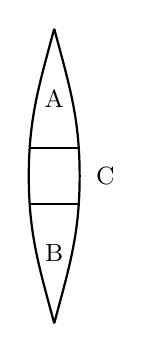
\begin{tikzpicture}[scale=0.85,font=\small]
  % Biconvex lens with central strip C marked
  \draw[thick] (0, 2.2) to[out=-105,in=90] (-0.38, 0) to[out=-90,in=105] (0, -2.2);
  \draw[thick] (0, 2.2) to[out=-75,in=90] (0.38, 0) to[out=-90,in=75] (0, -2.2);
  % Horizontal cuts for C
  \draw[thick] (-0.36, 0.42) -- (0.36, 0.42);
  \draw[thick] (-0.36, -0.42) -- (0.36, -0.42);
  \node at (0, 1.15) {A};
  \node at (0, -1.15) {B};
  \node[right] at (0.48, 0) {C};
\end{tikzpicture}
